\def\p{0.6}%
\def\centerx{0}%
\def\centery{0}%
\pgfplotsset{
    colormap={cool}{rgb255(0cm)=(255,255,255); rgb255(1cm)=(0,128,255); rgb255(2cm)=(255,0,255)}
}%
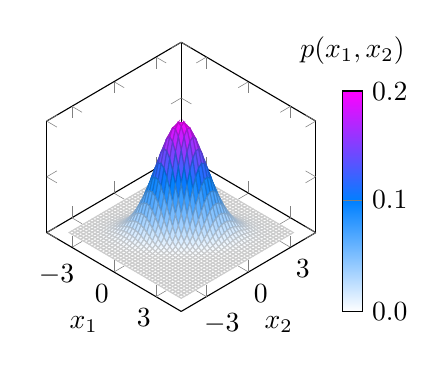
\begin{tikzpicture}
    \begin{axis}[
      width=5cm,height=5cm,
      xlabel=$x_1$,
      ylabel=$x_2$,
      xlabel shift={-10pt},
      ylabel shift={-10pt},
      zmin=0,
      zmax=0.2,
      domain=-4:4,
      enlarge x limits,
      enlarge y limits,
      scaled y ticks=false,
      scaled x ticks=false,
      xtick={-3, 0, 3},
      xticklabels={$-3$, $0$, $3$},
      ytick={-3, 0, 3},
      yticklabels={$-3$, $0$, $3$},
      zticklabels={},
      view={45}{45},
      colorbar,
      colormap name=cool,
      colorbar style={
        title={$p(x_1, x_2)$},
        ytick={0, 0.1, 0.197},
        yticklabels={$0.0$, $0.1$, $0.2$},
        height=2.8cm,
        at={(1.1,0)},
        anchor=south west
        % ylabel=$p(x_1, x_2)$
      },
      colorbar/width=2.5mm,
      ]%
      \addplot3[surf, samples=40, shader=faceted,thin]
      {1/(2 *pi* sqrt(1-\p^2))* exp(-((x-\centerx)^2+(y-\centery)^2-2*\p*(x-\centerx)*(y-\centery))/(2*(1-\p^2))};%
    \end{axis}
\end{tikzpicture}